\documentclass[a4paper, xelatex, ja=standard]{bxjsarticle}
% \setpagelayout*{top=25truemm,bottom=25truemm,left=25truemm,right=25truemm}

% パッケージインストール
\usepackage{plisting}
\usepackage{docmute}

% 文書開始
\begin{document}
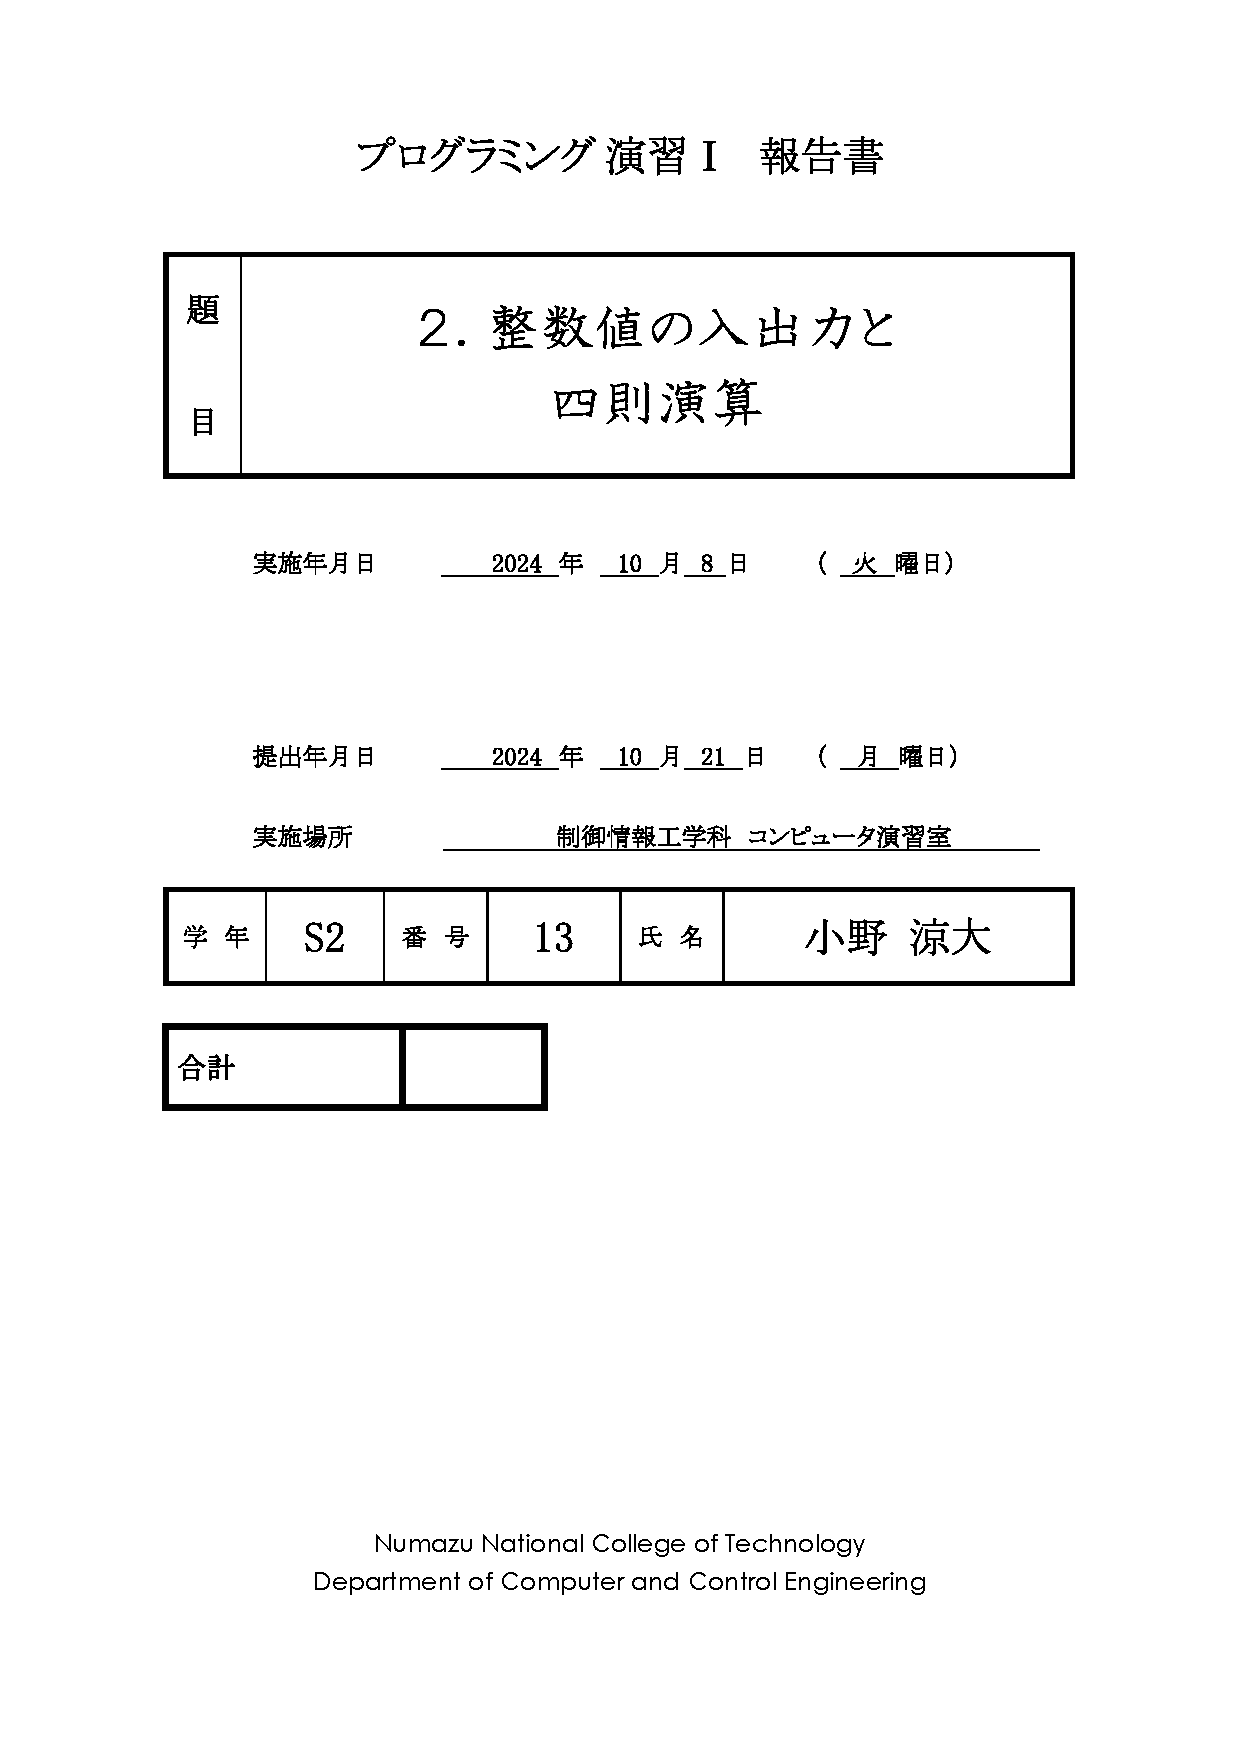
\includepdf{../cover.pdf}

\section{問題設定}
被乗数と乗数の2つの整数を端末から入力し,
その積を出力するプログラムを作成する.

\begin{lstlisting}[caption=例,label=]
[onosans@onosans-shyvana w02]$ ./ex.out
被乗数と乗数を入力してください
被乗数: 365
乗数: 17
365 x 17 = 6205
\end{lstlisting}

\section{問題分析}
今回の問題はまずユーザーに対しどのような値が欲しいのか示す必要がある.
そのため\texttt{printf}で「被乗数と乗数を入力してください」と出力する.

次に乗数, 被乗数の入力を受け付ける.
まず入力された値を一度メモリに保存する必要があるため
整数(int)型の変数を2つ宣言する.
次にどちらの値を受け付けるかなどの細かい表示をして,
\texttt{scanf}を使い先ほど宣言した変数に入力された値を代入する.

最後にそれらを計算した結果を出力すれば終了となる.


\section{設計}
今回作成するプログラムのフローチャートを以下に示す.

\begin{figure}[H]
\centering
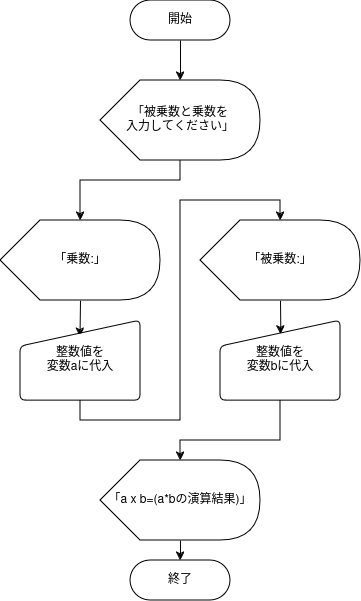
\includegraphics[scale=0.4]{../img/flowchart.drawio.png}
\caption{フローチャート}
\label{}
\end{figure}

\section{実装}
まず変数表を以下に載せる.

\begin{table}[h]
\centering
\caption{変数表}
\label{}
\begin{tabular}{|c|c|c|c|}
\hline
データ & 変数名                         & データ型 & 説明  \\ \hline
入力  & \texttt{a} & int  & 被乗数 \\ \hline
入力  & \texttt{b} & int  & 乗数  \\ \hline
\end{tabular}
\end{table}

それぞれの変数の役割は載せた表の通りである.
次に今回書いたコードを載せる.

\begin{lstlisting}[caption=ソースコード,label=s01]
#include <stdio.h>

int main(void){
	int a, b; // 整数型の変数a, bを宣言
	printf("被乗数と乗数を入力して下さい\n");
	printf("被乗数:");
	scanf("%d", &a); // aに入力された値を代入
	printf("乗数:");
	scanf("%d", &b); // bに入力された値を代入

	// 乗算した結果の出力
	printf("%d x %d = %d\n", a, b, a*b);

	return 0;
}
\end{lstlisting}

前回から使っているものの説明は省く.
\texttt{scanf}関数はターミナルからの入力を受け付ける関数である.
入力された値をどこの変数にどのような形式で保存するのかを,
第1引数に書式指定子, 第2引数に変数のメモリ上のアドレスを渡すことで
指定の変数に値を保存している.
10進数の場合, 書式指定子は\texttt{\%d},
変数のアドレスは変数名の前に\texttt{\&}をつける.

次に\texttt{printf}の新しい使い方として書式指定子を用いて
変数の値を代入する方法がある.
使い方はソースコード\ref{s01}のように
対応する場所に書式指定子を入れ,
対応する値(変数や演算)をコンマ区切りで入れていく.

これらの機能を使って以上のようにコードを組み立てた.

\section{検証}
実行結果は図\ref{fig:result}の通りである.
実行環境は前回と異なり, 
ArchLinuxで実行した.
\begin{figure}[h]
\centering
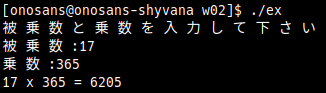
\includegraphics[scale=1.0]{../img/terminal_result.png}
\caption{実行結果}
\label{fig:result}
\end{figure}

\section{考察}
問題設定の通りのプログラムを書くことができた.
次にこのプログラムに対してバグを発生させる余地が残っているので
そちらを調べることと,
別の実装方法について考えてみた.

\subsection{オーバーフローさせてみる}
私の使用しているものも
\texttt{int}型のサイズは32bitのため
-2147483648から2147483647までの整数を表現することができる.
試しに2147483648と1を入力してみる.
すると結果は以下のようになる.
\begin{lstlisting}[caption=オーバーフロー1,label=]
[onosans@onosans-shyvana w02]$ ./ex.out
被乗数と乗数を入力してください
被乗数: 2147483648
乗数: 1
2147483648 x 1 = -2147483648
\end{lstlisting}

\begin{table}[h]
  \centering
  \caption{}
  \label{}
  \begin{tabular}{|c||c|c|}
  \hline
  & 10進数 & 2進数 \\ \hline
  被乗数 & 2147483648 & 1000 0000 0000 0000 0000 0000 0000 0000 \\ \hline
  答え & -2147483648(2の補数) & 1000 0000 0000 0000 0000 0000 0000 0000 \\ \hline
  \end{tabular}
\end{table}
このように2進数で見ても正しいことがわかる.
2の補数の仕組み上,
表現できる最大値の次の値は表現できる最小値になることを
改めて確認することができた.

これを回避するのであれば
\texttt{a}, \texttt{b}の符号を何らかの形で保存しておき
演算結果と符号を保存した変数の組み合わせを比べる.
もし演算結果の符号が正しくなければ「オーバーフローしました」
などと表示し再度入力を求めることで
このバグを回避することができるだろう.

\subsection{乗算を使わない実装}
乗算を使わずとも加算の繰り返しで
乗算と同じことをできるので,
加算の繰り返しによる実装を行った.
尚, 繰り返しの記述方法は既に知っていたので
参考文献には記述していない.
\begin{lstlisting}[caption=加算のみでの実装,label=]
#include <stdio.h>

int main(void){
	int a, b;
	printf("被乗数と乗数を入力して下さい\n");
	printf("被乗数:");
	scanf("%d", &a);
	printf("乗数:");
	scanf("%d", &b);

	int ans=0; // 積を保持する変数

	// b回繰り返し実行するという意味
	for(int i=0; i < b; i++){
		ans+=a; // ansにaの値を加算する
	}

	// 乗算した結果の出力
	printf("%d x %d = %d\n", a, b, ans);

	return 0;
}
\end{lstlisting}

\begin{table}[h]
\centering
\caption{変数表2}
\label{}
\begin{tabular}{|c|c|c|c|}
\hline
データ & 変数名 & データ型 & 説明  \\ \hline
出力 & \texttt{num} & int  & 演算途中の値の保存 \\ \hline
入力 & \texttt{a} & int  & 被乗数 \\ \hline
入力 & \texttt{b} & int  & 乗数  \\ \hline
\end{tabular}
\end{table}
こちらは乗数の回数分だけ加算を繰り返しているだけである.
今回の場合整数型なのでこれで実装することができているが,
浮動小数点型になった場合は1以下の部分については
被乗数を割れば実装できそうだがそもそも割り算をどう実装するのか
あまり思いついていない状況ではある.

\subsection{仮想的な乗算器を用いた実装}
ここからは完全に遊びなのだが
仮想的な乗算器を実装することによって,
今回のプログラムを作ってみようと思う.
ここでは乗算器のみ仮想的に実装するので
加算等は用いるが許してほしい.

また新たに使用した変数のみ
変数表にまとめた.
\begin{table}[h]
\centering
\caption{変数表3}
\label{}
\begin{tabular}{|c|c|c|c|}
\hline
データ & 変数名 & データ型 & 説明  \\ \hline
入力 & \texttt{a} & int  & 被乗数 \\ \hline
入力 & \texttt{b} & int  & 乗数  \\ \hline
内部 & \texttt{bool\_a[32]} & bool  & 被乗数を配列で表現  \\ \hline
内部 & \texttt{bool\_b[32]} & bool  & 乗数を配列で表現  \\ \hline
内部 & \texttt{n[32]} & int  & int型整数を配列で表すために使用する  \\ \hline
出力 & \texttt{p} & int  & 演算結果を格納する  \\ \hline
内部 & \texttt{q} & int  & 各桁ごとの演算結果を格納する  \\ \hline
内部 & \texttt{r} & int  & 桁同士の演算結果を格納する(イメージとしては\texttt{q}の手前)  \\ \hline
\end{tabular}
\end{table}

2の補数で表された数を式で書くなら以下のようになる.
\[
a = -a_{n-1}2^{n-1}+\sum_{i=0}^{n-2}a_i2^i
\]
ここで用いている$a_n$は$A$を2進数で表したときの
$n$bit目の値を表している(そのまま計算してもちゃんと-になるようにしてある).
この状態で加算を考えるなら以下のようになる.
\[
a \cdot b=(-a_{n-1}2^{n-1}+\cdots+a_12^1+a_02^0)(-b_{n-1}2^{n-1}+\cdots+b_12^1+b_02^0)
\]
マイナスのつく項をまとめると
\begin{align*}
-a_{n-1}b_02^{n-1}+-a_{n-1}b_12^{n}+\cdots+-a_{n-1}b_{n-2}2^{2n-3} \\
-a_0b_{n-1}2^{n-1}+-a_1b_{n-1}2^{n}+\cdots+-a_{n-2}b_{n-1}2^{2n-3}
\end{align*}
となっており, これらは
「各桁ごとの乗算の最後の値」と「最後の桁の乗算の最後以外の値」
に分類される.
これらをif文で条件分岐させ負の数にした後足し合わせることで
負の数の乗算も実装することができる.

実際に論理回路で実装する場合はビット反転ぐらいしかできないので,
このマイナスのつく値の部分を桁(後ろの2の指数)がかぶらないようにまとめると
ちょうどよく2つの組ができることがわかるだろう.
これらを2の補数で表し計算に組み込むことで実装できる.

いちいち2の補数にするといった動作をしていては効率が悪いので
一気に計算してみると
$n+1$bit目と$2n+1$bit目に1が加わることがわかる.
この1を実装すれば乗算器の完成だ.

C言語上で実装する場合,
ビット反転をしている方が追加で書く量や
変数も増えてしまうので
そのまま単純にマイナスをつけて実装している.
以下に機能ごとにソースコードを載せる.

最初にヘッダファイルの読み込みと
\texttt{main}関数を始めている.
\begin{lstlisting}[caption=最初の部分,label=]
#include <stdio.h>
#include <stdbool.h> // bool型を使えるようにする

int main(void){
\end{lstlisting}
\texttt{stdbool.h}を読み込むことで
\texttt{bool}型を使用できるようにしている.

次に入力された値を\texttt{bool}型の配列で
2進数として表現する.
\begin{lstlisting}[caption=\texttt{bool}型の配列で表す,label=]
// int型の変数を配列で表現するために使う変数の用意
int n[32];
for(int i=0; i<32; i++){
	n[i] = 1 << i;
}


// 入力値の保存
int a, b; // a: 被乗数 b: 乗数
printf("被乗数と乗数を入力して下さい\n");
printf("被乗数:");
scanf("%d", &a);
printf("乗数:");
scanf("%d", &b);


// bool型のa, b
bool bool_a[32], bool_b[32];

// aを配列で表現
for(int i=0; i < 32; i++){
	bool_a[i] = (a & n[i]) != 0;
}

// bを配列で表現
for(int i=0; i < 32; i++){
	bool_b[i] = (b & n[i]) != 0;
}
\end{lstlisting}
まず各bitごとに一つだけ1になっている
\texttt{int}型の配列\texttt{n}を用意する.
それらと\texttt{a}, \texttt{b}の論理和を取り
真だったとき配列のその場所を真, 偽であれば偽にする.
そうすることで\texttt{bool}型の配列で
\texttt{int}型の入力を表すことができる.

次に乗算している部分のコードを載せる.
\begin{lstlisting}[caption=乗算部,label=]
// 乗算に関する変数
int p=0, q, r; // p: 演算結果の保存 q: 各桁の合計 r: 各桁同士の演算結果の保存
for(int i=0; i < 32; i++){
	q=0;
	for(int j=0; j < 32; j++){
		r = ((int)(bool_a[i] && bool_b[j])) << j;
		// 各桁の最後の値or最後のbの最後のa以外を負の数にする
		if((j == 31 && i != 31) || (j != 31 && i == 31)){
			r = -r;
		}
		q += r;
	}
	q = q << i;
	p += q;
}
\end{lstlisting}
こちらではさきほど説明した演算方法を実行している.
各桁の論理積をとりその桁に合わせてビットシフトし
足しあわしている.
また負の数にも対応するために8行目のところで
条件分岐を入れ調節している.

最後に演算結果を出力している.
\begin{lstlisting}[caption=出力部,label=]
// 乗算結果の出力
printf("%d x %d = %d\n", a, b, p);

return 0;
\end{lstlisting}
これはソースコード\ref{s01}の出力部と
ほぼ一緒である.

\section{所感}
前回と違い2週間ほど時間もあり,
また土日も時間があったので
別の実装方法として色々考えてみた.
乗算器についてはもともと気になっていたので,
この機会に学習することができて良かった.

ただこれが本当に正しいのか確かめるために
総当りで普通に乗算したときの結果と比較することで,
ミスがないか確認している.
しかし, よくよく考えてみると$50\mbox{億}\times50\mbox{億}$程度の
計算量になっておりとても時間がかかっており, まだ終わっていない.
始めてしまったものは仕方ないのでしばらく動かしてみることにする.
他にいい方法があればそちらに切り替えようと考えているが,
今の所思いつかないので提出までに計算が終わればこちらに追記しておく.

\begin{thebibliography}{9}
\bibitem{key1} "乗算器". Wikipedia. 2024年6月1日. \url{https://ja.wikipedia.org/wiki/%E4%B9%97%E7%AE%97%E5%99%A8}, (\today).
\bibitem{key1} "符号付き2進数の乗算". Qiita. 2019年8月18日. \url{https://qiita.com/ryo_i6/items/f665a2267be6ba59c346}, (\today).
% \bibitem{key2} 符号拡張, \url{https://ja.wikipedia.org/wiki/%E7%AC%A6%E5%8F%B7%E6%8B%A1%E5%BC%B5}
\end{thebibliography}

\end{document}